\documentclass[pdflatex,sn-mathphys-num]{sn-jnl}
\usepackage{graphicx}
\usepackage{multirow}
\usepackage{amsmath,amssymb,amsfonts}
\usepackage{xcolor}
\usepackage{booktabs}
\usepackage{hyperref}
\usepackage{tikz}
\usetikzlibrary{positioning,arrows.meta,fit}
\usepackage[title]{appendix}

% All numbers below are generated from the result files by Code/make_manuscript_numbers.py.
% Generated by Code/make_manuscript_numbers.py -- do not edit by hand.
\newcommand{\biasHighHigh}{2.4}
\newcommand{\biasMedMed}{3.0}
\newcommand{\biasVLVL}{0.59$\times$}
\newcommand{\cohICclan}{7.5\%}
\newcommand{\cohICgo}{16.9\%}
\newcommand{\cohICgoRand}{5.6\%}
\newcommand{\cohIIclan}{26.4\%}
\newcommand{\cohIIgo}{57.7\%}
\newcommand{\cohIIgoRand}{24.8\%}
\newcommand{\cohRealClan}{6.7\%}
\newcommand{\cohRealGo}{19.8\%}
\newcommand{\cvFullRankAUC}{0.715}
\newcommand{\extBaseRate}{0.012}
\newcommand{\extBiomniP}{0.99}
\newcommand{\extBlendAUC}{0.670}
\newcommand{\extBlendPfive}{0.118}
\newcommand{\extBlendPooled}{0.733}
\newcommand{\extDegAUC}{0.558}
\newcommand{\extDotPfive}{0.089}
\newcommand{\extEsmHit}{40\%}
\newcommand{\extEsmPfive}{0.135}
\newcommand{\extEsmPooled}{0.595}
\newcommand{\extPerProtAUC}{0.653}
\newcommand{\extPerProtAUCesm}{0.650}
\newcommand{\extPooledAUC}{0.708}
\newcommand{\isoDevNoLink}{0}
\newcommand{\isoDevNoMatch}{240}
\newcommand{\isoDevNotSubmitted}{1{,}257}
\newcommand{\isoDevParalog}{153}
\newcommand{\isoFinalNoLink}{34}
\newcommand{\isoFinalNoMatch}{724}
\newcommand{\isoFinalNotSubmitted}{0}
\newcommand{\isoFinalParalog}{235}
\newcommand{\mapAgree}{98.6\%}
\newcommand{\nEdgesDev}{16{,}315}
\newcommand{\nEdgesFinal}{31{,}926}
\newcommand{\nExtLinks}{22{,}500}
\newcommand{\nExtProteins}{728}
\newcommand{\nExtProteinsWithLinks}{728}
\newcommand{\nIdentGroups}{111}
\newcommand{\nIdentProteins}{320}
\newcommand{\nIsoDev}{1{,}650}
\newcommand{\nIsoFinal}{993}
\newcommand{\nMappedFinal}{2{,}533}
\newcommand{\nNeverSubmitted}{1{,}257}
\newcommand{\nPfamAnnotated}{2{,}300}
\newcommand{\nPhmmerNew}{745}
\newcommand{\nProteins}{3{,}257}
\newcommand{\nSeeds}{10}
\newcommand{\nStringProteins}{2{,}642}
\newcommand{\nSubmitted}{2{,}000}
\newcommand{\nSurfaceProteins}{154}
\newcommand{\nWebMapped}{1{,}760}
\newcommand{\pOneBestGNN}{0.956\,$\pm$\,0.005}
\newcommand{\pOneBestGNNlabel}{Node2Vec with GCN}
\newcommand{\pOneBestHeur}{0.969\,$\pm$\,0.002}
\newcommand{\pOneBestHeurLabel}{resource allocation}
\newcommand{\pOneBiomni}{0.895\,$\pm$\,0.004}
\newcommand{\pOneRangeLow}{0.874}
\newcommand{\pThreeBest}{0.777\,$\pm$\,0.025}
\newcommand{\pThreeBestLabel}{Biomni+ESM-2+Node2Vec with MLP}
\newcommand{\pThreeBiomniGain}{+0.003}
\newcommand{\pThreeBiomniGainP}{0.037}
\newcommand{\pThreeBiomniOnly}{0.672\,$\pm$\,0.026}
\newcommand{\pThreeEsmMLP}{0.767\,$\pm$\,0.020}
\newcommand{\pThreeEsmRangeHigh}{0.777}
\newcommand{\pThreeEsmRangeLow}{0.767}
\newcommand{\pThreeNodeVecMax}{0.524}
\newcommand{\pThreePartnerDeg}{0.538\,$\pm$\,0.007}
\newcommand{\pThreeTiesMinP}{0.07}
\newcommand{\pTwoBest}{0.835\,$\pm$\,0.025}
\newcommand{\pTwoBestLabel}{Biomni+ESM-2 with MLP}
\newcommand{\pTwoPartnerDeg}{0.860\,$\pm$\,0.004}
\newcommand{\pctPfamAnnotated}{71\%}
\newcommand{\pyVersion}{3.12.9}
\newcommand{\pygVersion}{2.7.0}
\newcommand{\rMwLen}{0.999}
\newcommand{\sklearnVersion}{1.6.1}
\newcommand{\tierFracHigh}{3.0\%}
\newcommand{\tierFracMedium}{12.4\%}
\newcommand{\tierOR}{0.61}
\newcommand{\tierORp}{0.85}
\newcommand{\tierRho}{0.11}
\newcommand{\torchVersion}{2.9.1}
\newcommand{\vTwelveRecovered}{99.7\%}

% Items the authors must supply before submission are marked with \authorinput{...}.
\newcommand{\authorinput}[1]{\textcolor{red}{[AUTHOR INPUT: #1]}}

\raggedbottom

\begin{document}

\title[Cold-start interaction prediction for reverse vaccinology]{Sequence embeddings, not network topology, predict interactions of uncharacterized proteins: a leakage-aware benchmark with external validation for reverse vaccinology in \textit{Flavobacterium}}

\author[1]{\fnm{Muhammad} \sur{Kazim}}
\equalcont{These authors contributed equally to this work.}
\author[1]{\fnm{Faria} \sur{Farzana}}
\equalcont{These authors contributed equally to this work.}
\author*[1]{\fnm{Harun} \sur{Pirim}}\email{harun.pirim@ndsu.edu}
\equalcont{These authors contributed equally to this work.}
\author[2]{\fnm{Larry} \sur{Hanson}}
\author[2]{\fnm{Matt} \sur{Griffin}}
\author[3]{\fnm{Caitlin E.} \sur{Older}}
\author[3]{\fnm{Geoffrey C.} \sur{Waldbieser}}
\author[4]{\fnm{Thomas P.} \sur{Loch}}
\author[5]{\fnm{Benjamin R.} \sur{LaFrentz}}
\author[6]{\fnm{Esteban} \sur{Soto}}
\author[2]{\fnm{Hasan} \sur{Tekedar}}

\affil*[1]{\orgdiv{Department of Industrial \& Manufacturing Engineering}, \orgname{North Dakota State University}, \orgaddress{\city{Fargo}, \state{ND}, \country{USA}}}
\affil[2]{\orgdiv{College of Veterinary Medicine}, \orgname{Mississippi State University}, \orgaddress{\city{Mississippi State}, \state{MS}, \country{USA}}}
\affil[3]{\orgdiv{Warmwater Aquaculture Research Unit}, \orgname{United States Department of Agriculture, Agricultural Research Service}, \orgaddress{\city{Stoneville}, \state{MS}, \country{USA}}}
\affil[4]{\orgdiv{Aquatic Animal Health Laboratory}, \orgname{Michigan State University}, \orgaddress{\city{East Lansing}, \state{MI}, \country{USA}}}
\affil[5]{\orgdiv{Aquatic Animal Health Research Unit}, \orgname{United States Department of Agriculture, Agricultural Research Service}, \orgaddress{\city{Auburn}, \state{AL}, \country{USA}}}
\affil[6]{\orgdiv{Department of Medicine and Epidemiology, School of Veterinary Medicine}, \orgname{University of California, Davis}, \orgaddress{\city{Davis}, \state{CA}, \country{USA}}}

\abstract{\textbf{Background:} Reverse vaccinology for bacterial fish pathogens increasingly combines protein prioritization with interaction networks, and graph neural networks (GNNs) are often proposed to predict missing protein--protein associations. For non-model pathogens, the proteins of greatest interest frequently have no recorded interactions, yet link-prediction models are usually evaluated on randomly held-out edges between well-connected proteins, with uniformly sampled negatives. It is therefore unclear which inputs carry signal in the setting where such models are actually used.

\textbf{Results:} We built a homology-transferred STRING~v12 network for the \textit{Flavobacterium} sp.\ MO\_0223\_q7L1K proteome (\nProteins{} proteins, \nEdgesFinal{} associations) and benchmarked three GNN encoders and a graph-free multilayer perceptron with Biomni agent-derived descriptors, ESM-2 protein language model embeddings and Node2Vec embeddings under three protocols, with \nSeeds{} repeated splits each. On randomly held-out edges, parameter-free neighbourhood heuristics (ROC-AUC \pOneBestHeur) matched or exceeded every GNN (best \pOneBestGNN). When whole proteins were held out, Node2Vec fell to chance, and with uniform negatives the degree of the partner protein alone (\pTwoPartnerDeg) outperformed every trained model. With degree-matched negatives, all configurations combining ESM-2 with a graph-free encoder performed best and were statistically indistinguishable (ROC-AUC \pThreeEsmRangeLow--\pThreeEsmRangeHigh); no GNN improved on them. We validated this protocol externally on \nExtProteins{} proteins whose STRING links had been withheld by an upload limit (\nExtLinks{} links): pooled ROC-AUC was \extPooledAUC{}, matching the internal estimate (\cvFullRankAUC), and for per-protein partner lists plain ESM-2 nearest neighbours were the best pre-specified ranking (precision@5 \extEsmPfive{} versus \extBaseRate{} at random). Biomni priority tiers were not enriched for outer-membrane, TonB-dependent or type~IX secretion families (High versus other tiers: odds ratio \tierOR{}), and tier homophily in predicted links reflected model bias rather than the recovered interactions.

\textbf{Conclusions:} For proteins without known interactions, sequence embeddings provide the usable signal and graph structure provides none; evaluation protocol, not architecture, determined the apparent ranking of methods. We release a leakage-aware benchmark, an externally validated candidate list for \nIsoFinal{} interaction-orphan proteins, and an audit of agent-derived vaccine priorities to support reverse vaccinology in \textit{Flavobacterium}.}

\keywords{Reverse vaccinology, Link prediction, Graph neural networks, Protein language models, Cold-start evaluation, \textit{Flavobacterium}, Aquaculture}

\maketitle

%======================================================================
\section{Background}\label{sec:background}
%======================================================================

\textit{Flavobacterium} species cause some of the most damaging bacterial diseases of farmed freshwater fish, including columnaris disease (\textit{F.\ columnare}) and bacterial cold-water disease (\textit{F.\ psychrophilum}), and effective vaccines remain limited by incomplete knowledge of protective antigens \cite{gomez2014f,hoare2017efficacy,cai2021deciphering}. Reverse vaccinology addresses this by ranking proteins from genome sequence for properties associated with protective immunity, such as surface exposure, secretion and conservation \cite{sunita2020computational,bravi2024development,rawal2021identification}. In \textit{Flavobacterium}, the type~IX secretion system (T9SS) is required for virulence and exports adhesins, peptidases and toxins bearing conserved C-terminal sorting domains \cite{li2017t9ss,barbier2020t9ss,thunes2021t9ss}, making secreted and outer-membrane proteins natural candidates.

Protein--protein association networks add biological context to such rankings, but they are incomplete and biased towards well-studied proteins \cite{szklarczyk2023string,szklarczyk2025string}. Link prediction, and in particular graph neural networks (GNNs) such as GCN, GAT and GraphSAGE \cite{kipf2017gcn,velickovic2018gat,hamilton2017inductive}, has been proposed to infer missing associations, including for proteins without any known partner. Two well-documented evaluation problems make reported performance difficult to interpret for that use. First, randomly splitting edges leaves both proteins of almost every test pair in the training graph; performance on such pairs does not transfer to pairs involving unseen proteins \cite{park2012flaw}, and models evaluated this way learn largely from sequence similarity and node degree \cite{bernett2024cracking}. Second, uniformly sampled negative pairs are easy to separate from positives on degree alone, so simple heuristics often match GNNs \cite{li2023linkpitfalls,dunham2021benchmark}. Recent work further indicates that, once leakage is controlled, the signal in sequence-based interaction prediction comes mostly from protein language model (PLM) embeddings rather than from the downstream architecture \cite{reim2025plateau}.

Reverse vaccinology pipelines increasingly also rely on AI agents for protein annotation. Biomni is a general-purpose biomedical agent \cite{huang2025biomni} that can produce per-protein physicochemical descriptors and priority scores, but the reliability of agent-derived priorities as antigen predictors has not been assessed against independent evidence.

Here we ask which inputs predict associations for proteins that have none recorded, using the proteome of a \textit{Flavobacterium} isolate. We (i) benchmark Biomni descriptors, ESM-2 embeddings \cite{lin2023esm2} and Node2Vec embeddings \cite{grover2016node2vec} with three GNN encoders, a graph-free encoder and non-learned baselines under protocols that do and do not hold out whole proteins and control for degree; (ii) validate the held-out-protein protocol externally on proteins whose associations were withheld from the development network; (iii) audit Biomni priority tiers against Pfam families of surface and secreted proteins chosen in advance; and (iv) release a ranked, annotated candidate list for proteins without interaction evidence.

%======================================================================
\section{Methods}\label{sec:methods}
%======================================================================

\subsection{Proteome, sequence groups and functional annotation}
The study used the predicted proteome of \textit{Flavobacterium} sp.\ MO\_0223\_q7L1K (\nProteins{} proteins; RAST annotation, \authorinput{genome accession / BioProject and isolation source}). \nIdentProteins{} proteins fall into \nIdentGroups{} groups of identical sequence; members of a group receive identical features, so identical pairs were excluded from all candidate lists and external evaluation, and per-protein lists were collapsed to one representative per group. Protein domains were annotated with Pfam~38.2 \cite{paysanlafosse2025pfam} using pyhmmer \cite{larralde2023pyhmmer} (HMMER3 \cite{eddy2011hmmer}) with the curated gathering thresholds; domains were mapped to clans and to Gene Ontology terms with pfam2go. \nPfamAnnotated{} proteins (\pctPfamAnnotated) carried at least one domain.

\subsection{Biomni descriptors and priority tiers}
For every protein, Biomni \cite{huang2025biomni} produced a signal-peptide score, the number of predicted transmembrane segments, cysteine content, GRAVY hydrophobicity, length, molecular weight, instability index, isoelectric point and a composite vaccine score, from which four priority tiers were assigned (Very Low $<0.3$, Low $0.3$--$0.45$, Medium $0.5$--$0.65$, High $\geq0.7$) \authorinput{Biomni version, run date, language-model backbone, prompts and the generated code, to be released as Supplementary File S1}. Because molecular weight and length are almost perfectly correlated ($r=\rMwLen$), molecular weight was dropped; the number of transmembrane segments and length were log-transformed, and all descriptors were standardised to zero mean and unit variance before modelling (node descriptors contain no edge information, so standardisation over all proteins does not leak test labels).

\subsection{Protein language model embeddings}
Each sequence was embedded with ESM-2 \cite{lin2023esm2} (650M parameters, \texttt{esm2\_t33\_650M\_UR50D}; 1,280 dimensions) by averaging final-layer residue representations, excluding special tokens. Sequences longer than 1,022 residues were split into consecutive chunks and all residues were averaged. The 35M-parameter model (480 dimensions) was used as a sensitivity analysis (Supplementary Table~\ref{tab:esm_size}).

\subsection{Interaction networks}\label{sec:networks}
\textit{Flavobacterium} sp.\ MO\_0223\_q7L1K is not represented in STRING, so associations were transferred by homology from \textit{F.\ columnare} ATCC~49512 (STRING taxon 1041826, STRING v12 \cite{szklarczyk2023string}). Two networks were used (Table~\ref{tab:data}).

\emph{Development network.} The STRING web interface accepts at most 2,000 sequences; the \nSubmitted{} longest proteins had been submitted, \nWebMapped{} were mapped by STRING, and the exported associations (combined score $\geq0.4$) formed a network of \nEdgesDev{} edges in which \nIsoDev{} proteins had no edge, \nNeverSubmitted{} of them because they were never submitted. All model development and selection used this network.

\emph{Final network.} All \nProteins{} proteins were searched against the \nStringProteins{} STRING~v12 proteins of taxon 1041826 with phmmer, keeping the best hit with a bit score at least as high as the weakest mapping STRING itself had accepted (51.2 bits). This mapping agreed with the STRING web mapping for \mapAgree{} of the \nWebMapped{} proteins and mapped \nPhmmerNew{} of the \nNeverSubmitted{} never-submitted proteins. Each STRING protein was assigned to its highest-scoring proteome match (lower-scoring paralogous matches remain without edges to avoid duplicating edge sets between near-identical proteins), and links with combined score $\geq400$ were retained, giving \nEdgesFinal{} edges and \nIsoFinal{} proteins without edges. The development network's edges are a subset of the final network (\vTwelveRecovered{} recovered), confirming that the original export also came from STRING~v12.

\subsection{Models and baselines}
Three GNN encoders (GCN \cite{kipf2017gcn}, GAT \cite{velickovic2018gat}, GraphSAGE \cite{hamilton2017inductive}) and a graph-free two-layer perceptron (MLP) mapped node features to 64-dimensional embeddings (hidden size 128, dropout 0.5; GAT with four heads in the first layer), and pairs were scored with a dot-product decoder. Models were trained with binary cross-entropy and Adam (learning rate $10^{-3}$, at most 60 epochs, early stopping on validation ROC-AUC with patience 12) in PyTorch Geometric. Seven feature sets combined Biomni descriptors, ESM-2 embeddings and Node2Vec embeddings. Node2Vec \cite{grover2016node2vec} (128 dimensions, $p=q=1$, 80 walks of length 10 per node, window 5) was refitted for every split on training edges only. Non-learned baselines were common neighbours, Adamic--Adar, resource allocation and preferential attachment \cite{liben2003link,lu2011link}, the degree of the partner protein in the training graph, and the cosine similarity of ESM-2 embeddings.

\subsection{Evaluation protocols}\label{sec:protocols}
Each protocol used \nSeeds{} random splits (seeds 0--9) and the same splits for every model and feature set (Fig.~\ref{fig:design}).

\emph{P1, edge split.} Edges were split 80/10/10 into training, validation and test sets with an equal number of uniformly sampled non-edges as negatives; both proteins of a test pair generally remain in the training graph.

\emph{P2, held-out proteins with uniform negatives.} 10\% of connected proteins were held out for validation and 10\% for testing together with all their edges, so that at evaluation time they have no edges in the message-passing graph, exactly like interaction-orphan proteins. Test positives are edges between a test protein and a training protein (class C2 of Park and Marcotte \cite{park2012flaw}); pairs of two test proteins (C3) are reported separately. Negatives were uniform random non-edges with the same node-type constraint.

\emph{P3, held-out proteins with degree-matched negatives.} As P2, but each endpoint of a negative pair was sampled in proportion to its frequency among positive pairs, so that degree alone cannot separate positives from negatives \cite{li2023linkpitfalls}.

We report ROC-AUC and average precision (mean $\pm$ s.d.\ over splits). Each configuration was compared with the best one by paired $t$-tests and Wilcoxon signed-rank tests over splits, with Benjamini--Hochberg correction across the family of comparisons.

\subsection{External validation on withheld proteins}\label{sec:external}
Proteins that were never submitted to STRING but are mappable to STRING~v12 provide associations that no model saw during development. For each such protein that is isolated in the development network, we scored all candidate partners (all connected proteins and the other isolated proteins, excluding identical sequences and pairs mapped to the same STRING protein) with the models trained on the development network and compared the rankings with its STRING~v12 links (combined score $\geq400$). Metrics were per-protein ROC-AUC, precision among the five top-ranked partners (P@5), whether a true partner appears among the top ten, and pooled ROC-AUC and precision across all pairs.

\subsection{Candidate scoring and re-ranking}
Final scores were averaged over the ten models trained on the P3 splits, using the configuration selected on the development network (Biomni+ESM-2, MLP encoder; it is within the statistically tied group on the final network). Because dot-product scores favour a few partners with large embedding norms, five ranking variants were declared before evaluation: the raw score; cosine similarity of model embeddings; a hubness-corrected cosine (CSLS, $k=10$) \cite{conneau2018csls}; ESM-2 cosine similarity; and rank blends of the model cosine with ESM-2 cosine. The variant with the highest mean per-protein P@5 on the internal P3 test proteins was pre-selected; all variants were then evaluated once on the external set.

\subsection{Biological evaluation}
Six sets of Pfam families associated with surface exposure or secretion were fixed in advance by accession (T9SS C-terminal sorting domains, outer-membrane proteins, TonB-dependent/SusCD uptake systems, T9SS and gliding machinery, adhesin and surface-repeat domains, type~VI secretion; Supplementary Table~\ref{tab:families}). Enrichment of these families by Biomni tier was tested with Fisher's exact test (High versus other tiers) and Spearman correlation with tier rank. Functional coherence of predicted pairs was measured as the fraction of pairs (both proteins annotated) sharing a Pfam family, a Pfam clan or a GO term, compared with 50,000 random candidate pairs and with all edges of the final network. Tier-pair composition of predictions was compared with that of the recovered STRING links of the external proteins.

\subsection{Software and reproducibility}
Analyses used Python~\pyVersion, PyTorch~\torchVersion, PyTorch Geometric~\pygVersion, scikit-learn~\sklearnVersion, gensim~4.4.0, fair-esm~2.0.0 and pyhmmer~0.12.3. All code, configuration files, per-split indices, results tables and the candidate lists are released (see Data availability).

\begin{figure}[t]
\centering
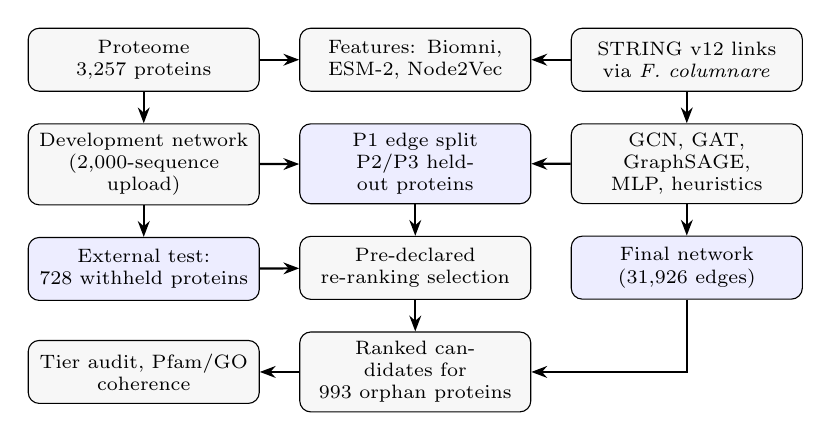
\begin{tikzpicture}[font=\scriptsize, node distance=4mm and 5mm,
  box/.style={draw, rounded corners, align=center, minimum height=8mm, text width=27mm, fill=gray!6},
  hl/.style={box, fill=blue!7},
  arr/.style={-{Stealth[length=2mm]}, thick}]
\node[box] (prot) {Proteome\\\nProteins{} proteins};
\node[box, right=of prot] (feat) {Features: Biomni,\\ESM-2, Node2Vec};
\node[box, right=of feat] (net) {STRING v12 links\\via \textit{F.\ columnare}};
\node[box, below=of prot] (dev) {Development network\\(2,000-sequence upload)};
\node[hl, below=of feat] (prot3) {P1 edge split\\P2/P3 held-out proteins};
\node[box, below=of net] (models) {GCN, GAT, GraphSAGE,\\MLP, heuristics};
\node[hl, below=of dev] (ext) {External test:\\\nExtProteins{} withheld proteins};
\node[box, below=of prot3] (sel) {Pre-declared\\re-ranking selection};
\node[hl, below=of models] (final) {Final network\\(\nEdgesFinal{} edges)};
\node[box, below=of sel] (cand) {Ranked candidates for\\\nIsoFinal{} orphan proteins};
\node[box, left=of cand] (bio) {Tier audit, Pfam/GO\\coherence};
\draw[arr] (prot) -- (feat); \draw[arr] (net) -- (feat);
\draw[arr] (prot) -- (dev); \draw[arr] (dev) -- (prot3); \draw[arr] (models) -- (prot3);
\draw[arr] (dev) -- (ext); \draw[arr] (prot3) -- (sel); \draw[arr] (ext) -- (sel);
\draw[arr] (net) -- (models); \draw[arr] (models) -- (final);
\draw[arr] (final) |- (cand); \draw[arr] (sel) -- (cand); \draw[arr] (cand) -- (bio);
\end{tikzpicture}
\caption{Study design. Models and ranking choices were developed on the network built from the original 2,000-sequence STRING upload; proteins withheld by the upload limit served as an external test set; the final network built from all proteins was used for the reported benchmark and the released candidate list.}
\label{fig:design}
\end{figure}

\begin{table}[t]
\centering
\caption{Data used in this study.}
\label{tab:data}
\begin{tabular}{lrr}
\toprule
 & Development network & Final network \\
\midrule
Proteins (nodes) & \nProteins & \nProteins \\
Proteins mapped to STRING v12 & \nWebMapped & \nMappedFinal \\
Edges (combined score $\geq400$) & \nEdgesDev & \nEdgesFinal \\
Proteins without edges & \nIsoDev & \nIsoFinal \\
\quad not submitted to STRING & \isoDevNotSubmitted & \isoFinalNotSubmitted \\
\quad no STRING match & \isoDevNoMatch & \isoFinalNoMatch \\
\quad lower-scoring paralogue of a mapped protein & \isoDevParalog & \isoFinalParalog \\
\quad mapped, but no link with score $\geq400$ & \isoDevNoLink & \isoFinalNoLink \\
\bottomrule
\end{tabular}
\end{table}

%======================================================================
\section{Results}\label{sec:results}
%======================================================================

\subsection{On random edge splits, neighbourhood heuristics match or beat GNNs}
Under the edge-split protocol P1, every GNN configuration reached ROC-AUC of at least \pOneRangeLow{} (Fig.~\ref{fig:benchmark}a), and Biomni descriptors alone reached \pOneBiomni{}. Yet the best parameter-free heuristic (\pOneBestHeurLabel, \pOneBestHeur) matched or exceeded the best GNN configuration (\pOneBestGNNlabel, \pOneBestGNN). Because both proteins of nearly every test pair keep other edges in the training graph, this protocol measures how well a model reproduces local network structure, which simple heuristics already capture.

\subsection{Holding out proteins removes all topological signal and exposes degree bias}
When whole proteins were held out (P2), the topological methods failed as expected: neighbourhood heuristics scored exactly 0.5 because held-out proteins have no neighbours, and Node2Vec features were at or below chance with GCN and GAT (Fig.~\ref{fig:benchmark}b). With uniformly sampled negatives, however, ranking pairs by the degree of the training-graph partner reached \pTwoPartnerDeg{} ROC-AUC and outperformed every trained model (best \pTwoBestLabel, \pTwoBest). Uniform negatives therefore mostly reward predicting that new proteins attach to hubs.

With degree-matched negatives (P3), partner degree fell to \pThreePartnerDeg{} and Node2Vec to chance (Fig.~\ref{fig:benchmark}c, Table~\ref{tab:coldstart}). The remaining signal came from sequence embeddings: the four feature sets containing ESM-2 reached \pThreeEsmRangeLow--\pThreeEsmRangeHigh{} with the graph-free MLP (best \pThreeBestLabel, \pThreeBest; ESM-2 alone \pThreeEsmMLP), and their differences were not significant after correction (BH-adjusted Wilcoxon $p\geq\pThreeTiesMinP$). Node2Vec alone stayed at chance (at most \pThreeNodeVecMax), Biomni descriptors alone reached \pThreeBiomniOnly, and adding Biomni descriptors to ESM-2 changed ROC-AUC by \pThreeBiomniGain{} (paired Wilcoxon $p=\pThreeBiomniGainP$, uncorrected). For every feature set containing ESM-2, the graph-free MLP was at least as good as any GNN encoder. ESM-2 650M was marginally better than the 35M model (Supplementary Table~\ref{tab:esm_size}).

\begin{figure*}[t]
\centering
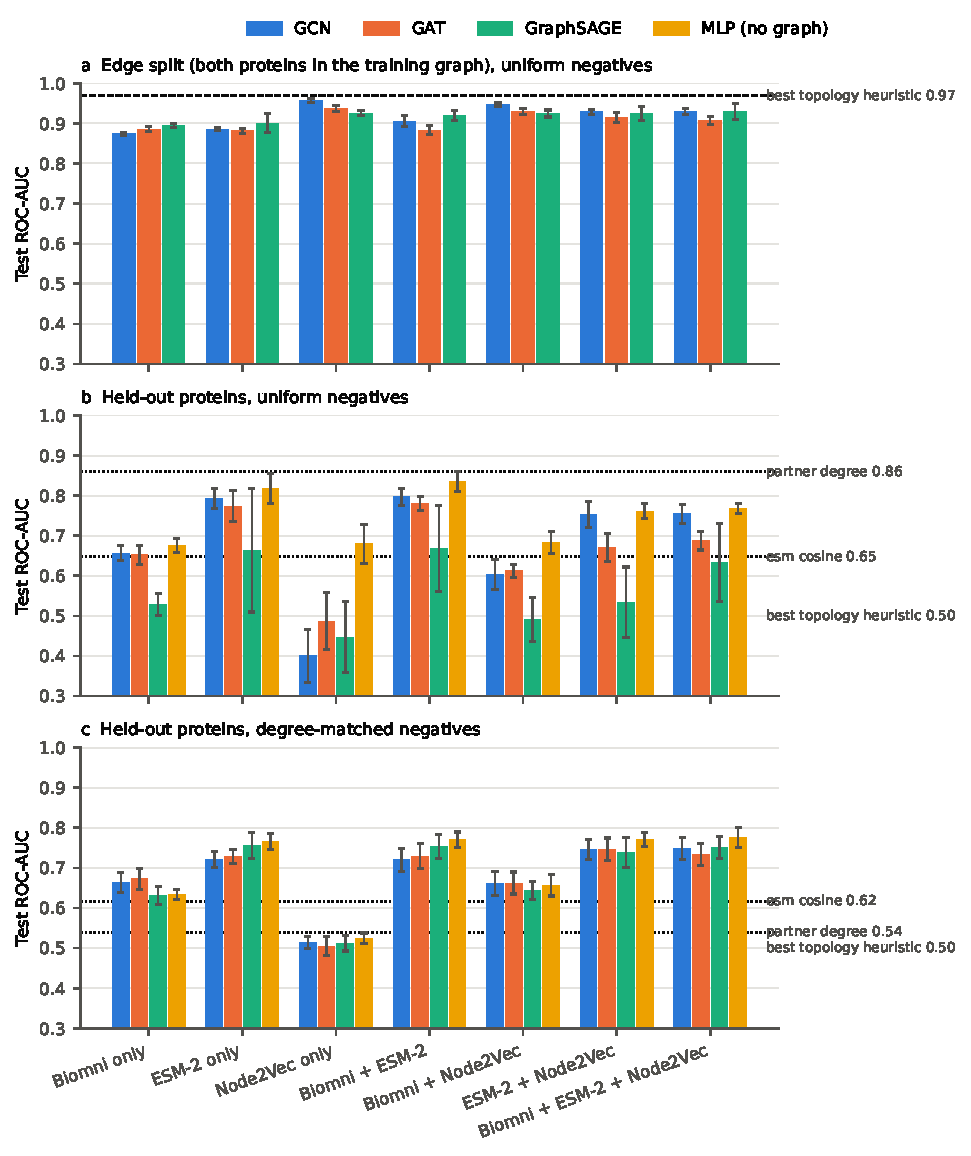
\includegraphics[width=0.95\textwidth]{figures/fig_benchmark.pdf}
\caption{Benchmark on the final network (\nSeeds{} splits; bars, mean test ROC-AUC; whiskers, s.d.). (a)~P1, random edge split with uniform negatives (GNN encoders only). (b)~P2, held-out proteins with uniform negatives (test pairs between a held-out and a training protein). (c)~P3, held-out proteins with degree-matched negatives. Horizontal lines mark non-learned baselines.}
\label{fig:benchmark}
\end{figure*}

\begin{table}[t]
\centering
\caption{Held-out proteins with degree-matched negatives (P3), final network. Test ROC-AUC, mean $\pm$ s.d.\ over \nSeeds{} splits; best value per row in bold.}
\label{tab:coldstart}
{\footnotesize\setlength{\tabcolsep}{2.5pt}\begin{tabular}{lcccc}
\toprule
Feature set & GCN & GAT & GraphSAGE & MLP \\
\midrule
Biomni & 0.663\,$\pm$\,0.024 & \textbf{0.672\,$\pm$\,0.026} & 0.631\,$\pm$\,0.023 & 0.633\,$\pm$\,0.013 \\
ESM-2 & 0.721\,$\pm$\,0.020 & 0.729\,$\pm$\,0.017 & 0.756\,$\pm$\,0.032 & \textbf{0.767\,$\pm$\,0.020} \\
Node2Vec & 0.514\,$\pm$\,0.014 & 0.505\,$\pm$\,0.023 & 0.512\,$\pm$\,0.019 & \textbf{0.524\,$\pm$\,0.014} \\
Biomni+ESM-2 & 0.721\,$\pm$\,0.029 & 0.729\,$\pm$\,0.031 & 0.753\,$\pm$\,0.030 & \textbf{0.770\,$\pm$\,0.020} \\
Biomni+Node2Vec & 0.662\,$\pm$\,0.030 & \textbf{0.662\,$\pm$\,0.028} & 0.645\,$\pm$\,0.022 & 0.657\,$\pm$\,0.027 \\
ESM-2+Node2Vec & 0.746\,$\pm$\,0.025 & 0.747\,$\pm$\,0.028 & 0.738\,$\pm$\,0.037 & \textbf{0.771\,$\pm$\,0.018} \\
Biomni+ESM-2+Node2Vec & 0.748\,$\pm$\,0.028 & 0.733\,$\pm$\,0.026 & 0.751\,$\pm$\,0.027 & \textbf{0.777\,$\pm$\,0.025} \\
\midrule
Best topology heuristic & \multicolumn{4}{c}{0.500\,$\pm$\,0.000} \\
Partner degree & \multicolumn{4}{c}{0.538\,$\pm$\,0.007} \\
ESM-2 cosine similarity & \multicolumn{4}{c}{0.617\,$\pm$\,0.007} \\
\bottomrule
\end{tabular}
}
\end{table}

\subsection{External validation confirms the held-out-protein estimate}
\nExtProteinsWithLinks{} proteins that were isolated in the development network only because they were never submitted to STRING have \nExtLinks{} STRING~v12 links to candidate partners (base rate \extBaseRate). Scored by models trained before these links were known, they gave a pooled ROC-AUC of \extPooledAUC{} (Table~\ref{tab:external}, Fig.~\ref{fig:external}), in line with the internal P3 estimate for the same model and network (\cvFullRankAUC), and well above partner degree (\extDegAUC). Biomni descriptors did not improve on ESM-2 alone in this set (per-protein ROC-AUC \extPerProtAUC{} versus \extPerProtAUCesm; Wilcoxon $p=\extBiomniP$).

Per-protein partner lists were dominated by a few partners with large embedding norms (raw-score P@5 \extDotPfive). Among the pre-declared re-ranking variants, ESM-2 nearest neighbours had the highest internal P@5 and were therefore pre-selected; externally they again gave the best partner lists (P@5 \extEsmPfive, a true partner in the top ten for \extEsmHit{} of proteins), but the worst pooled ranking (ROC-AUC \extEsmPooled). Blending model cosine with ESM-2 cosine gave the best per-protein ROC-AUC (\extBlendAUC) with intermediate P@5 (\extBlendPfive) and pooled ROC-AUC \extBlendPooled. The internal ordering of variants predicted the external ordering, supporting the use of P3 for model selection.

\begin{table}[t]
\centering
\caption{External validation on \nExtProteinsWithLinks{} proteins withheld from the development network (\nExtLinks{} STRING~v12 links). Models were trained on the development network (Biomni+ESM-2 unless stated).}
\label{tab:external}
{\footnotesize\setlength{\tabcolsep}{2.5pt}\begin{tabular}{lccccc}
\toprule
Ranking & \multicolumn{3}{c}{Per protein} & \multicolumn{2}{c}{Pooled} \\
\cmidrule(lr){2-4}\cmidrule(lr){5-6}
 & AUC & P@5 & Hit@10 & AUC & P@0.1\% \\
\midrule
Model, Biomni+ESM-2 & 0.653 & 0.089 & 0.216 & 0.708 & 0.195 \\
Model, ESM-2 only & 0.650 & 0.091 & 0.221 & 0.721 & 0.356 \\
ESM-2 cosine (pre-selected) & 0.638 & 0.135 & 0.404 & 0.595 & 0.059 \\
Blend (0.5) & 0.670 & 0.118 & 0.353 & 0.733 & 0.199 \\
Partner degree & 0.547 & 0.090 & 0.317 & 0.558 & 0.105 \\
Random & 0.500 & 0.012 & -- & 0.500 & 0.012 \\
\bottomrule
\end{tabular}
}
\end{table}

\begin{figure*}[t]
\centering
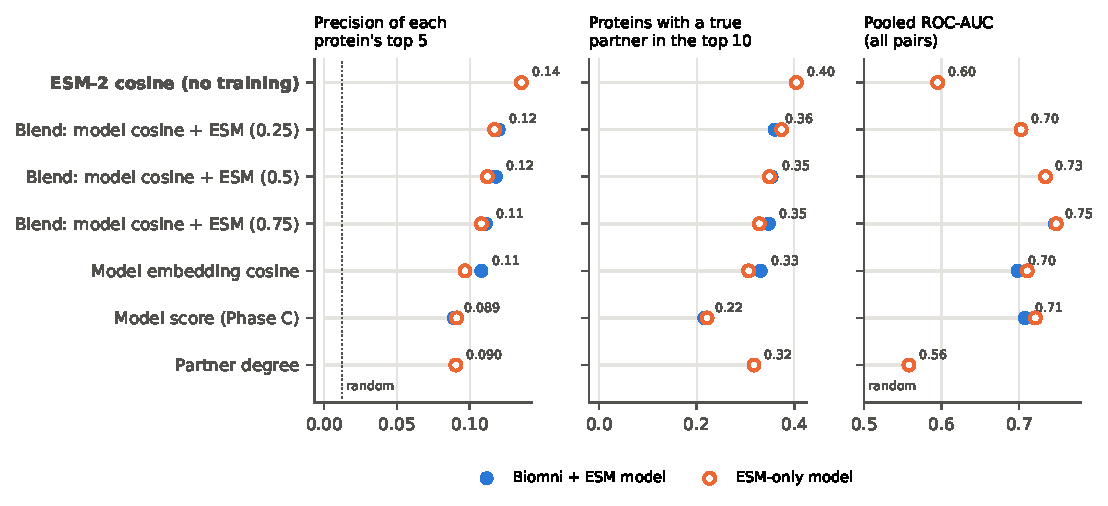
\includegraphics[width=0.95\textwidth]{figures/fig_external_validation.pdf}
\caption{External validation of ranking variants. Filled markers, Biomni+ESM-2 model; open markers, ESM-2-only model. The bold variant was selected in advance on the internal P3 splits. Dotted lines, random expectation.}
\label{fig:external}
\end{figure*}

\subsection{Biomni priority tiers do not single out surface or secreted protein families}
Of the \nSurfaceProteins{} proteins carrying a pre-specified surface or secretion family, the highest fraction fell in the Medium tier (\tierFracMedium) rather than the High tier (\tierFracHigh; Fig.~\ref{fig:tiers}a). High-tier proteins were not enriched for these families (odds ratio \tierOR{}, BH-adjusted $p=\tierORp$); the weak positive trend over tiers (Spearman $\rho=\tierRho$) was carried by the Medium tier, and no TonB-dependent or SusCD protein was ranked High.

In the model's top predictions, pairs of Medium- and High-tier proteins were over-represented relative to the candidate pool. The external set shows that this is not a property of the true associations: compared with the recovered STRING links of the same proteins, the model's top-five partners over-represented Medium--Medium pairs \biasMedMed-fold and High--High pairs \biasHighHigh-fold, and under-represented Very Low--Very Low pairs (\biasVLVL; Fig.~\ref{fig:tiers}b). Tier homophily in predicted links should therefore not be read as biological evidence.

\begin{figure*}[t]
\centering
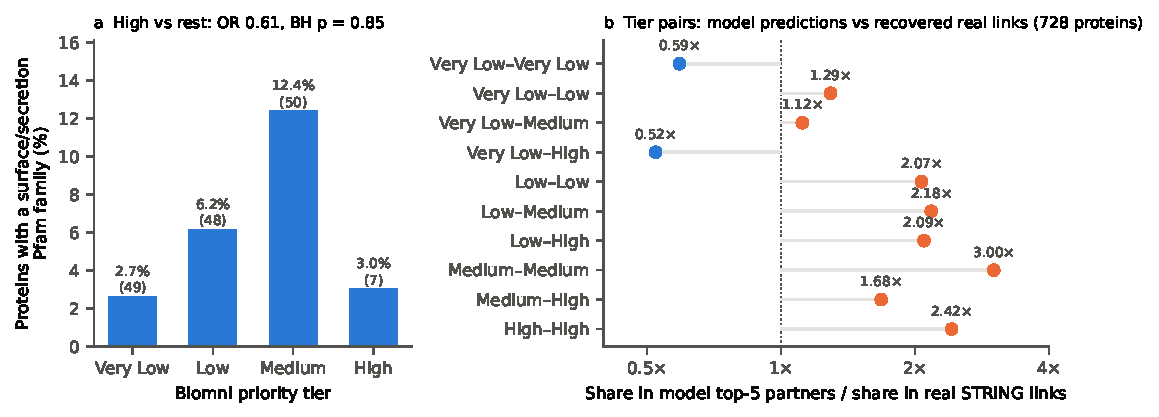
\includegraphics[width=0.95\textwidth]{figures/fig_biomni_tiers.pdf}
\caption{Audit of Biomni priority tiers. (a)~Fraction of proteins carrying a pre-specified surface or secretion Pfam family, by tier (counts in parentheses). (b)~Tier-pair composition of the model's top-five partners relative to the recovered STRING~v12 links of the same \nExtProteinsWithLinks{} external proteins.}
\label{fig:tiers}
\end{figure*}

\subsection{Predicted partners are functionally coherent}
On the final network, the top 2,000 predicted pairs (at most five per protein) shared a GO term (\cohICgo{} for isolated--connected and \cohIIgo{} for isolated--isolated pairs) and a Pfam clan (\cohICclan{} and \cohIIclan) far more often than random candidate pairs (\cohICgoRand{} and \cohIIgoRand{} for GO terms; all BH-adjusted $p<0.001$), at rates comparable to the edges of the network itself (\cohRealGo{} GO, \cohRealClan{} clan), and higher for isolated--isolated pairs (Fig.~\ref{fig:coherence}). Because ESM-2 embeddings encode homology, part of this coherence reflects sequence similarity, and it supports plausibility rather than independent confirmation. The released candidate list covers the \nIsoFinal{} proteins without edges in the final network, annotated with Pfam domains, GO terms, Biomni descriptors and identical-sequence groups.

\begin{figure}[t]
\centering
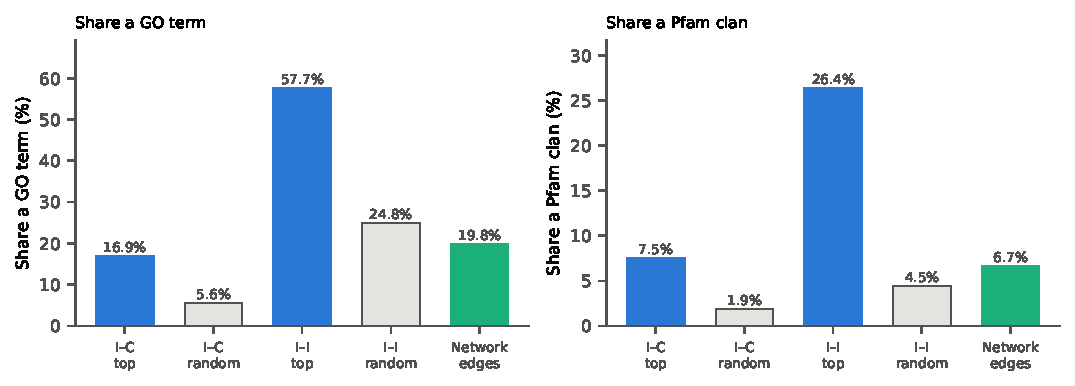
\includegraphics[width=\columnwidth]{figures/fig_coherence.pdf}
\caption{Functional coherence of the top 2,000 predicted pairs on the final network (at most five per protein) compared with random candidate pairs and with the network's own edges. I--C, isolated--connected pairs; I--I, isolated--isolated pairs.}
\label{fig:coherence}
\end{figure}

%======================================================================
\section{Discussion}\label{sec:discussion}
%======================================================================

The ranking of methods in this study was determined by the evaluation protocol rather than by model architecture. On random edge splits, GNNs were matched or outperformed by neighbourhood-counting heuristics; with whole proteins held out but uniform negatives, a degree heuristic beat every model; and only with degree-matched negatives did a stable picture emerge, in which sequence embeddings carried the signal and graph structure carried none. These observations agree with general analyses of link-prediction and pair-input evaluation \cite{park2012flaw,li2023linkpitfalls,bernett2024cracking} and with the finding that PLM embeddings account for most of the attainable performance in leakage-controlled interaction prediction \cite{reim2025plateau}. For reverse vaccinology, where the proteins of interest are often exactly those without recorded interactions, the practical implication is that network-topology methods add nothing for such proteins and that reported performance must come from a held-out-protein protocol with degree-controlled negatives.

The external validation is the most direct test of this protocol. Because the upload limit withheld the associations of \nNeverSubmitted{} proteins from the development network, models could be scored on associations that no step of development had seen, and the internal estimate (\cvFullRankAUC) matched the external result (\extPooledAUC). The same set showed that the best tool for a per-protein partner list was the simplest: nearest neighbours in ESM-2 space. Trained models remain useful for ranking pairs across proteins, which matters when deciding which predictions to follow up, and blending the two gives a balanced ranking. We report the pre-declared choice together with the alternatives so that users can select the ranking suited to their purpose.

Biomni descriptors added at most a marginal amount of information to ESM-2 internally and none externally, and the priority tiers derived from them did not identify the outer-membrane, TonB-dependent and T9SS cargo families that dominate the \textit{Flavobacterium} virulence literature \cite{li2017t9ss,thunes2021t9ss}. Agent-derived priority scores are convenient, but they encode heuristic weightings whose behaviour should be audited against independent annotation before they are used to select antigens. Releasing the agent's version, prompts and generated code is necessary for such outputs to be reproducible.

Several limitations apply. Associations were transferred from a related strain, so they inherit both the coverage of \textit{F.\ columnare} in STRING and the uncertainty of homology transfer; STRING associations are functional, not necessarily physical. The external set consists of proteins withheld for a technical reason, and they are shorter on average than the submitted ones; their associations include conserved complexes such as the ribosome, which are easier to predict than those of typical antigen candidates. ESM-2 similarity partly encodes homology, so functional coherence of predictions is evidence of plausibility rather than of novel biology. Finally, the analysis covers one proteome and makes no claim about transfer to other pathogens, and no prediction has been tested experimentally; the candidate list is a set of ranked hypotheses for follow-up.

%======================================================================
\section{Conclusions}\label{sec:conclusions}
%======================================================================

For proteins without known interactions in a non-model fish pathogen, protein language model embeddings provide the usable signal for association prediction, graph topology provides none, and agent-derived vaccine priorities do not track independent surface and secretion annotations. A held-out-protein protocol with degree-matched negatives gave performance estimates that held on externally withheld proteins. We release the benchmark, code and an annotated candidate list as a reproducible basis for reverse vaccinology in \textit{Flavobacterium}.

\backmatter

\bmhead{Supplementary information}
Supplementary Tables~A1--A4 are provided in the Appendix. Supplementary File~S1 documents the Biomni run \authorinput{to be supplied}.

\bmhead{Acknowledgements}
\authorinput{acknowledgements, including computing resources}.

\section*{Declarations}
\begin{itemize}
\item \textbf{Funding:} \authorinput{funding sources and grant numbers}.
\item \textbf{Competing interests:} The authors declare no competing interests.
\item \textbf{Ethics approval and consent to participate:} Not applicable; computational study of publicly available or author-generated bacterial sequence data.
\item \textbf{Data availability:} The proteome, both networks, mappings, Pfam/GO annotations, ESM-2 embeddings, per-split indices, all result tables and the candidate lists are available at \url{https://github.com/CEL-lab/USDA_Protein} \authorinput{archived release DOI (e.g.\ Zenodo) and genome accession}. STRING~v12 data are available from \url{https://string-db.org}.
\item \textbf{Code availability:} All analysis scripts are in the \texttt{Code/} directory of the repository above.
\item \textbf{Author contributions:} \authorinput{CRediT contributions}.
\end{itemize}

\begin{thebibliography}{99}

\bibitem{gomez2014f}
E.~G{\'o}mez, J.~M{\'e}ndez, D.~Cascales, and J.~A.~Guijarro,
``\textit{Flavobacterium psychrophilum} vaccine development: a difficult task,''
\emph{Microbial Biotechnology}, 7(5):414--423, 2014.

\bibitem{hoare2017efficacy}
R.~Hoare, T.~P.~H.~Ngo, K.~L.~Bartie, and A.~Adams,
``Efficacy of a polyvalent immersion vaccine against \textit{Flavobacterium psychrophilum} and evaluation of immune response to vaccination in rainbow trout fry (\textit{Onchorynchus mykiss} L.),''
\emph{Veterinary Research}, 48(1):43, 2017.

\bibitem{cai2021deciphering}
W.~Cai and C.~R.~Arias,
``Deciphering the molecular basis for attenuation of \textit{Flavobacterium columnare} strain Fc1723 used as modified live vaccine against columnaris disease,''
\emph{Vaccines}, 9(11):1370, 2021.

\bibitem{sunita2020computational}
Sunita, A.~Sajid, Y.~Singh, and P.~Shukla,
``Computational tools for modern vaccine development,''
\emph{Human Vaccines \& Immunotherapeutics}, 16(3):723--735, 2020.

\bibitem{bravi2024development}
B.~Bravi,
``Development and use of machine learning algorithms in vaccine target selection,''
\emph{npj Vaccines}, 9(1):15, 2024.

\bibitem{rawal2021identification}
K.~Rawal, R.~Sinha, B.~A.~Abbasi, A.~Chaudhary, S.~K.~Nath, P.~Kumari, P.~Preeti, D.~Saraf, S.~Singh, K.~Mishra \emph{et~al.},
``Identification of vaccine targets in pathogens and design of a vaccine using computational approaches,''
\emph{Scientific Reports}, 11(1):17626, 2021.

\bibitem{li2017t9ss}
N.~Li, Y.~Zhu, B.~R.~LaFrentz, J.~P.~Evenhuis, D.~W.~Hunnicutt, R.~A.~Conrad, P.~Barbier, C.~W.~Gullstrand, J.~E.~Roets, J.~L.~Powers \emph{et~al.},
``The type IX secretion system is required for virulence of the fish pathogen \textit{Flavobacterium columnare},''
\emph{Applied and Environmental Microbiology}, 83(23):e01769-17, 2017.

\bibitem{barbier2020t9ss}
P.~Barbier, T.~Rochat, H.~H.~Mohammed, G.~D.~Wiens, J.-F.~Bernardet, D.~Halpern, E.~Duchaud, and M.~J.~McBride,
``The type IX secretion system is required for virulence of the fish pathogen \textit{Flavobacterium psychrophilum},''
\emph{Applied and Environmental Microbiology}, 86(16):e00799-20, 2020.

\bibitem{thunes2021t9ss}
N.~C.~Thunes, R.~A.~Conrad, H.~H.~Mohammed, Y.~Zhu, P.~Barbier, J.~P.~Evenhuis, D.~Perez-Pascual, J.-M.~Ghigo, B.~R.~LaFrentz, and M.~J.~McBride,
``Type IX secretion system effectors and virulence of the model \textit{Flavobacterium columnare} strain MS-FC-4,''
\emph{Applied and Environmental Microbiology}, 88(3):e01705-21, 2022.

\bibitem{szklarczyk2023string}
D.~Szklarczyk, R.~Kirsch, M.~Koutrouli, K.~Nastou, F.~Mehryary, R.~Hachilif, A.~L.~Gable, T.~Fang, N.~T.~Doncheva, S.~Pyysalo \emph{et~al.},
``The STRING database in 2023: protein--protein association networks and functional enrichment analyses for any sequenced genome of interest,''
\emph{Nucleic Acids Research}, 51(D1):D638--D646, 2023.

\bibitem{szklarczyk2025string}
D.~Szklarczyk, K.~Nastou, M.~Koutrouli, R.~Kirsch, F.~Mehryary, R.~Hachilif, D.~Hu, M.~E.~Peluso, Q.~Huang, T.~Fang \emph{et~al.},
``The STRING database in 2025: protein networks with directionality of regulation,''
\emph{Nucleic Acids Research}, 53(D1):D730--D737, 2025.

\bibitem{kipf2017gcn}
T.~N.~Kipf and M.~Welling,
``Semi-supervised classification with graph convolutional networks,''
in \emph{International Conference on Learning Representations (ICLR)}, 2017.

\bibitem{velickovic2018gat}
P.~Veli{\v{c}}kovi{\'c}, G.~Cucurull, A.~Casanova, A.~Romero, P.~Li{\`o}, and Y.~Bengio,
``Graph attention networks,''
in \emph{International Conference on Learning Representations (ICLR)}, 2018.

\bibitem{hamilton2017inductive}
W.~Hamilton, Z.~Ying, and J.~Leskovec,
``Inductive representation learning on large graphs,''
\emph{Advances in Neural Information Processing Systems}, 30, 2017.

\bibitem{park2012flaw}
Y.~Park and E.~M.~Marcotte,
``A flaw in the typical evaluation scheme for pair-input computational predictions,''
\emph{Nature Methods}, 9(12):1134--1136, 2012.

\bibitem{bernett2024cracking}
J.~Bernett, D.~B.~Blumenthal, and M.~List,
``Cracking the black box of deep sequence-based protein--protein interaction prediction,''
\emph{Briefings in Bioinformatics}, 25(2):bbae076, 2024.

\bibitem{li2023linkpitfalls}
J.~Li, H.~Shomer, H.~Mao, S.~Zeng, Y.~Ma, N.~Shah, J.~Tang, and D.~Yin,
``Evaluating graph neural networks for link prediction: current pitfalls and new benchmarking,''
\emph{Advances in Neural Information Processing Systems}, 36, 2023.

\bibitem{dunham2021benchmark}
B.~Dunham and M.~Ganapathiraju,
``Benchmark evaluation of protein--protein interaction prediction algorithms,''
\emph{Molecules}, 27(1):41, 2021.

\bibitem{reim2025plateau}
T.~Reim, A.~Hartebrodt, D.~B.~Blumenthal, J.~Bernett, and M.~List,
``Deep learning models for unbiased sequence-based PPI prediction plateau at an accuracy of 0.65,''
\emph{Bioinformatics}, 2025.

\bibitem{huang2025biomni}
K.~Huang, S.~Zhang, H.~Wang, Y.~Qu, Y.~Lu, Y.~Roohani, R.~Li, L.~Qiu, G.~Li, J.~Zhang \emph{et~al.},
``Biomni: a general-purpose biomedical AI agent,''
\emph{bioRxiv}, 2025.

\bibitem{lin2023esm2}
Z.~Lin, H.~Akin, R.~Rao, B.~Hie, Z.~Zhu, W.~Lu, N.~Smetanin, R.~Verkuil, O.~Kabeli, Y.~Shmueli \emph{et~al.},
``Evolutionary-scale prediction of atomic-level protein structure with a language model,''
\emph{Science}, 379(6637):1123--1130, 2023.

\bibitem{grover2016node2vec}
A.~Grover and J.~Leskovec,
``node2vec: scalable feature learning for networks,''
in \emph{Proceedings of the 22nd ACM SIGKDD International Conference on Knowledge Discovery and Data Mining}, pp.~855--864, 2016.

\bibitem{paysanlafosse2025pfam}
T.~Paysan-Lafosse, A.~Andreeva, M.~Blum, S.~R.~Chuguransky, T.~Grego, B.~L.~Pinto, G.~A.~Salazar, M.~L.~Bileschi, F.~Llinares-L{\'o}pez, L.~Meng-Papaxanthos \emph{et~al.},
``The Pfam protein families database: embracing AI/ML,''
\emph{Nucleic Acids Research}, 53(D1):D523--D534, 2025.

\bibitem{larralde2023pyhmmer}
M.~Larralde and G.~Zeller,
``PyHMMER: a Python library binding to HMMER for efficient sequence analysis,''
\emph{Bioinformatics}, 39(5):btad214, 2023.

\bibitem{eddy2011hmmer}
S.~R.~Eddy,
``Accelerated profile HMM searches,''
\emph{PLoS Computational Biology}, 7(10):e1002195, 2011.

\bibitem{liben2003link}
D.~Liben-Nowell and J.~Kleinberg,
``The link prediction problem for social networks,''
in \emph{Proceedings of the Twelfth International Conference on Information and Knowledge Management}, pp.~556--559, 2003.

\bibitem{lu2011link}
L.~L{\"u} and T.~Zhou,
``Link prediction in complex networks: a survey,''
\emph{Physica A}, 390(6):1150--1170, 2011.

\bibitem{conneau2018csls}
A.~Conneau, G.~Lample, M.~Ranzato, L.~Denoyer, and H.~J{\'e}gou,
``Word translation without parallel data,''
in \emph{International Conference on Learning Representations (ICLR)}, 2018.

\end{thebibliography}

\begin{appendices}

\section{Supplementary tables}\label{sec:supp}

\begin{table}[h]
\centering
\caption{ESM-2 model size, development network, P3 (held-out proteins, degree-matched negatives). Test ROC-AUC, mean $\pm$ s.d.\ over \nSeeds{} splits.}
\label{tab:esm_size}
{\small\setlength{\tabcolsep}{3.5pt}\begin{tabular}{llcc}
\toprule
Feature set & Encoder & ESM-2 35M & ESM-2 650M \\
\midrule
ESM-2 & GraphSAGE & 0.710\,$\pm$\,0.026 & 0.716\,$\pm$\,0.027 \\
ESM-2 & MLP & 0.727\,$\pm$\,0.023 & 0.724\,$\pm$\,0.023 \\
Biomni+ESM-2 & GraphSAGE & 0.709\,$\pm$\,0.018 & 0.718\,$\pm$\,0.031 \\
Biomni+ESM-2 & MLP & 0.733\,$\pm$\,0.020 & 0.742\,$\pm$\,0.017 \\
ESM-2+Node2Vec & GraphSAGE & 0.705\,$\pm$\,0.037 & 0.730\,$\pm$\,0.027 \\
ESM-2+Node2Vec & MLP & 0.720\,$\pm$\,0.026 & 0.729\,$\pm$\,0.023 \\
Biomni+ESM-2+Node2Vec & GraphSAGE & 0.710\,$\pm$\,0.022 & 0.714\,$\pm$\,0.044 \\
Biomni+ESM-2+Node2Vec & MLP & 0.721\,$\pm$\,0.029 & 0.725\,$\pm$\,0.021 \\
ESM-2 cosine similarity & -- & 0.610\,$\pm$\,0.008 & 0.635\,$\pm$\,0.006 \\
\bottomrule
\end{tabular}
}
\end{table}

\begin{table}[h]
\centering
\caption{Pre-declared re-ranking variants: internal P3 test proteins (final network) and external validation (development network).}
\label{tab:rerank}
{\footnotesize\setlength{\tabcolsep}{2.5pt}\begin{tabular}{lcccccc}
\toprule
Variant & \multicolumn{3}{c}{Internal (final network)} & \multicolumn{3}{c}{External} \\
\cmidrule(lr){2-4}\cmidrule(lr){5-7}
 & P@5 & Prot.\ AUC & Pooled AUC & P@5 & Prot.\ AUC & Pooled AUC \\
\midrule
ESM-2 cosine & 0.125 & 0.646 & 0.601 & 0.135 & 0.638 & 0.595 \\
Blend cosine/ESM-2 (0.25) & 0.116 & 0.663 & 0.682 & 0.120 & 0.659 & 0.703 \\
Blend CSLS/ESM-2 (0.5) & 0.110 & 0.674 & 0.711 & 0.116 & 0.671 & 0.734 \\
Blend cosine/ESM-2 (0.5) & 0.109 & 0.673 & 0.711 & 0.118 & 0.670 & 0.733 \\
Blend cosine/ESM-2 (0.75) & 0.099 & 0.671 & 0.725 & 0.111 & 0.668 & 0.746 \\
Model cosine, CSLS & 0.086 & 0.660 & 0.693 & 0.107 & 0.661 & 0.701 \\
Model cosine & 0.084 & 0.659 & 0.690 & 0.108 & 0.660 & 0.698 \\
Model score & 0.079 & 0.654 & 0.712 & 0.089 & 0.653 & 0.708 \\
\bottomrule
\end{tabular}
}
\end{table}

\begin{table}[h]
\centering
\caption{Pfam family sets fixed in advance for the biological evaluation.}
\label{tab:families}
\begin{tabular}{lp{0.62\textwidth}}
\toprule
Family set & Pfam families \\
\midrule
T9SS cargo (CTD) & Por\_Secre\_tail (PF18962), CHU\_C (PF13585) \\
Outer membrane protein & OmpA (PF00691), OmpA\_like (PF16961), OMP\_b-brl\_3 (PF14905), OMP\_b-brl\_2 (PF13568), OMP\_b-brl (PF13505), OmpH (PF03938), OEP (PF02321), Omp85 (PF01103), Omp85\_2 (PF19143), POTRA (PF07244), Omp28 (PF11551), Toluene\_X (PF03349), LptD\_2 (PF19838), LptD\_N (PF03968), Gly-zipper\_Omp (PF13488), YfiO (PF13525) \\
TonB / SusCD uptake & Plug (PF07715), TonB\_dep\_Rec\_b-barrel (PF00593), SusD\_RagB (PF07980), SusD-like (PF12741), SusD-like\_2 (PF12771), SusD-like\_3 (PF14322), TonB\_C (PF03544) \\
T9SS / gliding machinery & PorP\_SprF (PF11751), PorV (PF19572), T9SS\_plug\_1st (PF17116), SprA\_N (PF14349), SprB (PF13573), GldM\_3rd (PF21602), GldM\_2nd (PF21601), GldM\_4th (PF12080), GldM\_1st (PF12081), GldL\_N (PF22827), GldN (PF19841), GldB\_lipo (PF25594), GldD\_lipo (PF25593), GldH\_lipo (PF14109), GldC-like (PF19937) \\
Adhesin / surface repeat & DUF2807 (PF10988), Cleaved\_Adhesin (PF07675), Big\_5 (PF13205), PKD (PF00801), PKD\_4 (PF18911), fn3 (PF00041), Laminin\_G\_3 (PF13385), RHS\_repeat (PF05593) \\
T6SS (type VI secretion) & TssD (PF17642), TssN (PF17555), TssO (PF17561), TssC (PF17541) \\
\bottomrule
\end{tabular}

\end{table}

\begin{table}[h]
\centering
\caption{Surface and secretion family sets by Biomni priority tier (fraction of proteins in each tier; Fisher test High versus other tiers, BH-adjusted).}
\label{tab:tiers}
{\small\setlength{\tabcolsep}{3.5pt}\begin{tabular}{lrccccc}
\toprule
Family set & $n$ & Very Low & Low & Medium & High & OR High (BH $p$) \\
\midrule
T9SS cargo (CTD) & 43 & 0.6\% & 2.2\% & 3.5\% & 0.4\% & 0.31 (0.85) \\
Outer membrane protein & 44 & 0.8\% & 0.9\% & 4.7\% & 1.7\% & 1.32 (0.96) \\
TonB / SusCD uptake & 31 & 0.5\% & 1.9\% & 1.7\% & 0.0\% & 0 (0.85) \\
T9SS / gliding machinery & 21 & 0.2\% & 0.6\% & 2.7\% & 0.4\% & 0.66 (1.00) \\
Adhesin / surface repeat & 14 & 0.2\% & 0.9\% & 0.7\% & 0.4\% & 1.01 (1.00) \\
T6SS (type VI secretion) & 13 & 0.6\% & 0.3\% & 0.0\% & 0.0\% & 0 (1.00) \\
Any surface/secretion family & 154 & 2.7\% & 6.2\% & 12.4\% & 3.0\% & 0.61 (0.85) \\
\bottomrule
\end{tabular}
}
\end{table}

\end{appendices}

\end{document}
